\subsection{Entity-Relationship Schema}
\begin{figure}[h!]
    \centering
    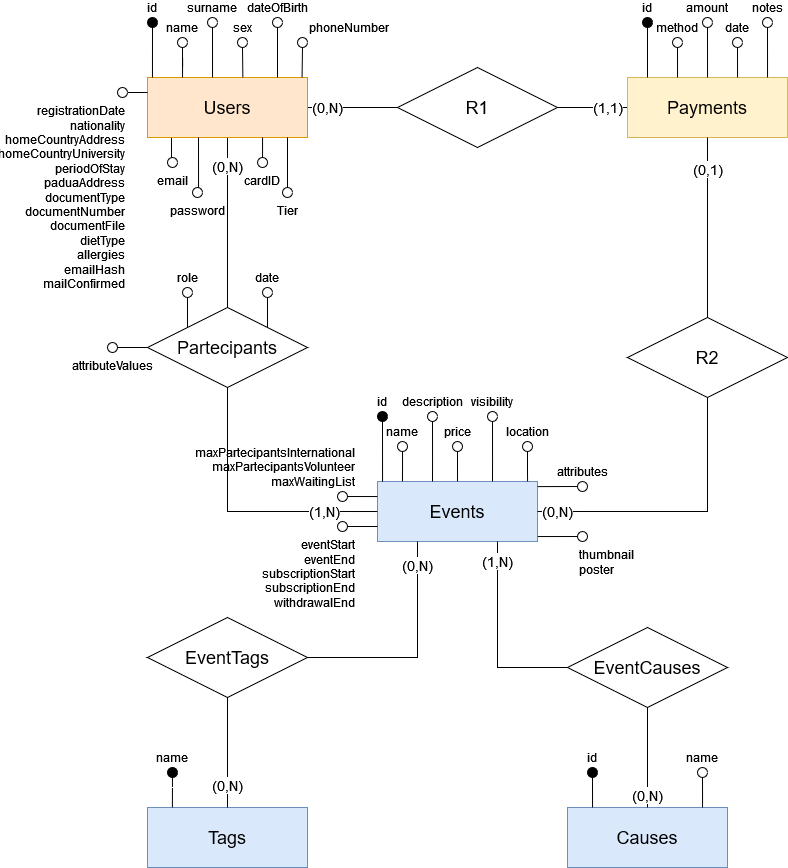
\includegraphics[width=1\textwidth]{images/ERSchema.png}
    \caption{Database ER schema}
    \label{fig:er_schema}
\end{figure}
Our database has 3 main entities, plus an important relation. Others are auxiliary
and will explained shortly at the end. Except only one entity, all entities has an integer ID
as primary key. Main entities are:
\begin{itemize}
    \item \textbf{Users:} this entity contains all the information about every kind of users, from
    tier 0 to system admin. This table has new entries every time registration form is filled: the dummy
    form will generate a tier 0 user, while the real form will generate a tier 1 user. Every attribute 
    is self-explanatory and stored in a very intuitive way: name and surname are varchar(50), all dates
    are type date with local time zone and so on.\\
    Here, just as examples, some attributes with their SQL code and few information about them.
\begin{lstlisting}[language=SQL]
CREATE TYPE diet AS ENUM ('No specific', 'Vegetarian',
                        'Vegan', 'Halal', 'Kosher', 'Pescetarian');

CREATE TABLE public."Users" (
id SERIAL PRIMARY KEY,
email VARCHAR(255) NOT NULL UNIQUE CHECK 
        email ~* '^[A-Za-z0-9._%+-]+@[A-Za-z0-9.-]+\.[A-Za-z]{2,}$'),
...
"homeCountryAddress" json,
...
"documentFile" text,
"dietType" diet,
)
\end{lstlisting}
    In the above snippet, we can see few special features: RegExpr is used to check mail spelling,
    addresses and similar variables are stores as json, for an easier data access. Diet and others
    are stored as enum, to avoid user typo and having more readable attributes. %TODO: images!!!!
    \item \textbf{Events:} as for users entity, event has a long list of attributes, wisely chosen
    in relation how events are actually organized. Some events are restricted to certain users, based
    on tiers, or have a limited number of participants. All these particularities are fully represented
    in the entity.
    \item \textbf{Payment:} this entity contains all the information about payment for event participation.
    Of course the actual web application isn't linked to real payment methods, but once il will be, this Entity
    will be related to real payments, in order to tracing them, know most favorite payment methods etc.
    \item \textbf{Participants:} opposed to previous entities, this is a relation between users and events,
    collecting user role, as listed in this snippet:
\begin{lstlisting}
CREATE TYPE roleTypes AS ENUM ('Organizer', 'Participant',
                            'Volunteer', 'WaitingList');
\end{lstlisting}
    Furthermore, date helps managing waiting list and attributes %TODO: why is it needed?
\end{itemize}